% !TeX program = xelatex
\documentclass[UTF8,11pt]{ctexart}

\usepackage{amsthm}
\usepackage{amsfonts}
\usepackage{amsmath}
\usepackage{float} % H
\usepackage{cite} % citation
\newtheorem{theorem}{定理}
\newtheorem{example}{例}
\usepackage{graphicx}
\usepackage{geometry}
\geometry{scale=0.8}
\usepackage{setspace}

\begin{document}
	\title{数学分析与线性代数例题}
	\author{佚名}
	\date{2019 年 12 月 6 日}
	\maketitle
	
	\tableofcontents
	\renewcommand{\baselinestretch}{1.8}

	\section{\songti 微分中值定理及其应用}
	\vspace{-1ex}
	    \begin{theorem}[极值的第二充分条件]
			 设$f(x)$在$(x_0-\delta,x_0+\delta)$可导且$f'(x_0)=0$,又$f''(x_0)$存在.
			 
			 1) 若 $f''(x_0)>0$,则 $f(x_0)$是严格极大值;

			 2) 若 $f''(x_0)<0$,则 $f(x_0)$是严格极小值;
	    \end{theorem}
		\begin{example}
			求$y=\frac{1}{3}\sqrt[3]{(x-5)^2}$的极值点与极值\footnote{原题摘自《数学分析简明教程》(上册)P142.1}.\\
			解. 函数在$(-\infty,+\infty)$上连续,当$x\not=5$时有
			\vspace{-4ex}
			\begin{equation}
			\vspace{-4ex}
				y'=\frac{1}{3}\Big((x-5)^\frac{2}{3} + \frac{2x}{3}(x-5)^{-\frac{1}{3}})=\frac{5(x-3)}{9(x-5)^\frac{1}{3}}\,.
			\end{equation}
			令$y'=0$得稳定点$x=3$,现列表如下:

			\begin{table}[H]
			\begin{center}
			\begin{tabular}{|c|c|c|c|c|c|}\hline
				$x$ & $(-\infty,3)$ & $3$ & $(3,5)$ & $5$ & $(5,+\infty)$\\\hline
				$y'$ & $+$ & $0$ & $-$ & $不存在$ & $+$\\\hline
				$y'$ & $\nearrow$ & $\sqrt[3]{4}$ & $\searrow$ & $0$ & $\nearrow$\\\hline
			\end{tabular}
			\end{center}
			\end{table}
			\vspace{-4ex}

			从表中可见$x=3$是极大值点,极大值为$f(3)=\sqrt[3]{4}$;$x=5$为极小值点,极小值为$f(5)=0$.我们可以大致地画出函数的图形,如图\ref{fig:function}所示.
			\begin{figure}[ht]
			\centering
			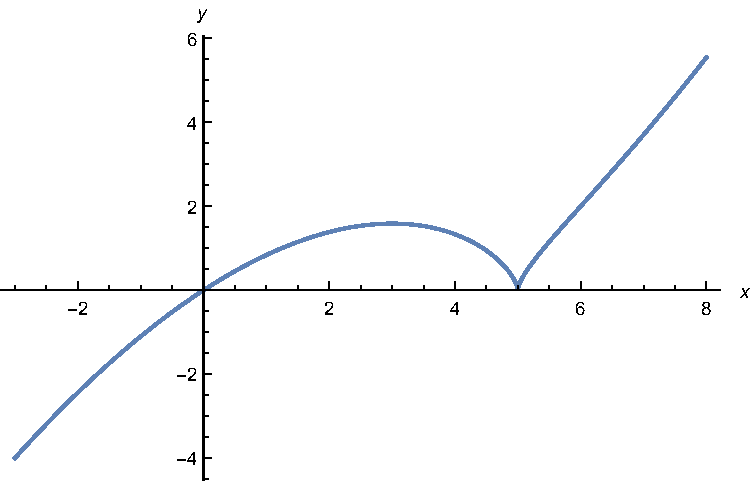
\includegraphics{function.pdf}
			\caption{\small\it $y=\frac{1}{3}x\sqrt[3]{(x-5)^2}$的函数图像}
			\label{fig:function}
			\end{figure}
		\end{example}

	\section{行列式}
		\begin{example}
			若$a,b\in\mathbb{R}^+$,求由方程为$\frac{x_1^2}{a^2}+\frac{x_2^2}{b^2}=1$的椭圆为边界的区域$E$的面积\footnote{原题摘自《线性代数及其应用》(第三版)P183.}.\\
			\textbf{解. }断言$E$是单位圆盘$D$在线性变换$T$下的像.这里$T$由矩阵$A=$
			$\begin{bmatrix}
				a & 0\\
				0 & b
			\end{bmatrix}$
			确定,这是因为若$\textbf{u}=$
			$\begin{bmatrix}
				u_1 \\
				u_2
			\end{bmatrix}$
			,$\textbf{x}=$
			$\begin{bmatrix}
				x_1 \\
				x_2
			\end{bmatrix}$
			,且$\textbf{x}=A\textbf{u}$,则
			\[u_1=\frac{x_1}{a} , u_2=\frac{x_2}{b}\]
			从而得\textbf{u}在此单位圆内,即满足$u_1^2+u_2^2\le1$,当且仅当$\textbf{x}$在$E$内,即满足$(x_1/a)^2+(x_2/b)^2\le1$.进而
			\begin{align*}
				\{\text{椭圆的面积}\}& =\{T(D)\text{的面积}\}\\
											 & =|det A|\cdot\{D\text{的面积}\}\\
											 & =a \cdot b \cdot \pi \cdot (1)^2\\
											 & =\pi ab
			\end{align*}
		\end{example}
	
	
\end{document}